
\begin{frame}
\frametitle{Image Locatization}
Second step:
\begin{itemize}
\item find bounding boxes of images on new books
\end{itemize}
\end{frame}

\subsection{Method}
\begin{frame}
\frametitle{Features}
Once again: HOG features
\end{frame}

\begin{frame}
\frametitle{Conditional Random Fields}
\begin{itemize}
\item What are CRFS?
\item Why CRFs?
\item Solver: SSVM
\end{itemize}
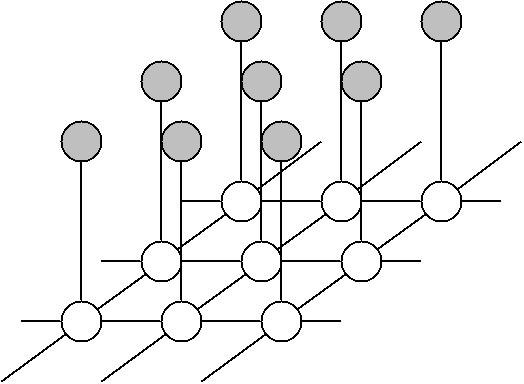
\includegraphics[width=.5\paperwidth]{resources/crf}
\end{frame}

\begin{frame}
\frametitle{Preprocess Features Using a SVM}
\begin{itemize}
\item HOG features have 8 values
\item SSVM has trouble with this
\item Use SVM to assign confidence score to each feature
\item Now SSVM has input of 1 value per feature
\end{itemize}
\end{frame}

\begin{frame}
\frametitle{Two Stage Training}
Require two stage training to prevent overfitting.
\begin{itemize}
\item Train SVM on $80\%$ of train set.
\item Predict labels using the trained SVM on other the $20\%$.
\item Repeat 5 times, with different splits
\item Now $100\%$ of data for SSVM is available
\item Once more: train SVM on $100\%$ of train set to obtain best model
\end{itemize}
\end{frame}

\subsection{Results}

\begin{frame}
\frametitle{Results}
insert results here
\end{frame}
